\documentclass[a5paper, 12dd, twoside]{article}
% !TeX spellcheck = ru_RU
%Автор - Краснов Александр 2022

%Настройка языка и отображения
\usepackage[russian]{babel}
%Шрифты
\usepackage[T2A]{fontenc}		%Русские шрифты
%\usefont{T2A}{Tempora-TLF}{m}{n}
%\usepackage{lmodern}			%Шрифт Latin Modern, нужен если нет cm-super

\usepackage[utf8]{inputenc}		%Кодировка
\usepackage{amssymb,amsmath}	%Математические символы
\usepackage{multicol}			%Несколько колонок
%\usepackage{color}				%Использовать цветной текст

\usepackage{graphicx}			%Пикчи
\DeclareGraphicsExtensions{.pdf,.png,.jpg}
\frenchspacing					%Отключает большой пробел между предложениями

\usepackage{indentfirst}		%Красная строка
\setlength{\parindent}{1.25cm}	%Настройка отступа красной строки для шрифта 14pt, по умолчанию 15pt
\linespread{1.25} 				%Межстрочный интервал

\usepackage{parskip} 			%Интервал между абзацами
\setlength{\parindent}{1cm} 	%Настройка интервала между абзацами, по умолчанию будет 0

\usepackage{enumitem}			%Настройка списков
\setlist{noitemsep}				%Убирает лишнюю строку в списках

\usepackage{textcomp}			%Улучшает знак номера

\usepackage{cmap}				%Ссылки в PDF
\usepackage[					%Гипертекстовое оглавление в PDF
bookmarks=true, colorlinks=true, unicode=true,
urlcolor=black,linkcolor=black, anchorcolor=black,
citecolor=black, menucolor=black, filecolor=black,
]{hyperref}

%\sloppy						%Автоматическое разряжение строк (только для черновиков)
\emergencystretch=20pt			%Аварийное разряжение строк (подбор опытным путем)
%\hfuzz=0.5pt					%Разрешить переполнение абзаца на 0.5dd (выглядит приемлемо)
\tolerance=300					%Настройка максимальной разряженности строки
\hyphenpenalty=100				%Настройка частоты переносов

\clubpenalty=5000				%Настройка висячих строк в начале абзаца от 0 до 10000
\widowpenalty=5000				%настройка висячих строк в конце абзаца от 0 до 10000


%Колонтитулы и номера страниц
%\pagestyle{empty} 				%Нет ни колонтитулов, ни номеров страниц
\pagestyle{plain} 				%Номера страниц ставятся внизу в середине строки, колонтитулов нет
%\pagestyle{headings} 			%Присутствуют колонтитулы (включающие в себя и номера страниц)
%\pagestyle{myheadings}			%То же, что и headings, но делается вручную

\pagenumbering{arabic}			%Нумерация страниц арабскими цифрами
%\pagenumbering{roman}			%Нумерация страниц римскими строчными цифрами
%\pagenumbering{Roman}			%Нумерация страниц римскими заглавными цифрами
%\pagenumbering{alph}			%Нумерация страниц строчными английскими буквами
%\pagenumbering{Alph}			%Нумерация страниц заглавными английскими буквами
%\pagenumbering{asbuk}			%Нумерация страниц строчными русскими буквами
%\pagenumbering{Asbuk}			%Нумерация страниц заглавными русскими буквами


%\usepackage{fancyhdr}			%Колонтитулы
%\pagestyle{fancy} 				%Использование кастомных колонтитулов
%\fancyhf{} 					%Отчистить все колонтитулы
%\lhead{} 						% левый верхний колонтитул
%\chead{} 						% центральный верхний
%\rhead{} 						% правый верхний
%\lfoot{} 						% левый нижний
%\cfoot{\thepage} 				% центральный нижний
%\rfoot{} 						% правый нижний


\usepackage{listings}
% настройка подсветки кода и окружения для листингов
%\usemintedstyle{colorful}
%\newenvironment{code}{\captionsetup{type=listing}}{}


%Спецсимволы
\usepackage{wasysym}			%Специальные символы, в том числе и гачи
\newcommand{\gachi}{\male}		%Гачи значок


%реализовать модификаторы шрифтов горячими клавишами



%Настройки верстки
%\openany						%Глава может начинаться с любой страницы
%\openright						%Глава только с правой страницы

%\fleqn							%Формулы слева
%\leqno							%Номера формул слева

%\raggedbottom					%Страницы разной высоты
\flushbottom					%Страницы одинаковой высоты

%\columnseprule=0.4pt			%Ширина линейки при верстке в колонки
%\columnsep=0mm					%Расстояние между колонками при верстке в колонки


%Настройка страниц

\usepackage[left=1.5cm, right=1.5cm, top=1.5cm, bottom=1.5cm]{geometry}
%twoside, openany,%
\hyphenation{
    про-из-вод-стве 
    до-пус-ти-мых 
    тех-но-ло-ги-чес-ких 
    рес-пи-ра-то-ров 
    про-вес-ти 
    э-лек-тро-маг-нит-но-го 
    ста-ти-сти-чес-ким 
    са-мо-сто-я-тель-но 
    ко-леб-лю-ще-го-ся 
    им-пульс-но-го 
    ус-та-нав-ли-ва-ют 
    не-пос-то-ян-но-го 
    ха-рак-те-рис-ти-ки
    про-из-вод-ствен-но-го 
    про-ме-жу-ток 
    пос-ле-ду-ю-щей
    раз-ве-ва-ю-щи-е-ся
    сви-са-ю-щи-е
    пред-ме-ты
    ре-зуль-та-те
    о-бес-то-чен
    за-кре-пи-те
    вни-ма-тель-ны
    и-зо-ля-ци-ю
    ком-плек-ту-ю-щи-е
    поз-во-ля-ет
    прак-ти-чес-ки
    об-ду-мать
    по-верх-нос-ти
    по-ло-же-ний
    по-лез-ность
    сто-ро-ной
    кон-струк-тив-но-го
    о-со-бен-нос-ти
    по-ни-ма-ния
    не-об-хо-ди-мые
    зна-ко-мых
    ис-поль-зу-ют-ся
    у-вле-ка-тель-ная
    ро-бо-то-тех-ни-ки
    у-прав-лять
    ин-струк-ци-ям
    у-да-лен-но
    функ-ци-о-наль-ность
    мо-ду-лю
    це-лом
    спе-ци-аль-нос-ти
    про-цесс
    об-щие
    по-лу-чи-ли
    ра-бо-та-ли
    тех-но-ло-ги-чес-кий
    ба-лан-си-ров-ки
    по-мощью
    ре-гу-ли-ру-ет-ся
    ско-рость
    от-но-си-тель-ную
    оп-ре-де-лять
    ком-пью-тер
    сиг-на-лы
    э-та-лон-ным
    пред-став-лен-но-го
    об-ра-зом
    пред-пи-сан-но-го
    пре-пят-ствий
    до-пол-ни-тель-ный
    преи-му-щест-ва
    кон-струк-ции
    за-клю-ча-ет-ся
    за-тра-ты
    на-мно-го
    сис-те-мах
    кон-ту-ру
    пе-ре-ход-ной
    ос-но-ве
    рас-сто-я-ние
    ос-лаб-ле-ние
    бла-го-да-ря
    за-мкну-то-му
    вы-со-кие
    ус-та-нов-ле-ния
    от-сле-жи-вать
    дат-чи-ка
    пред-став-лен-ный
    вклю-ча-ют
    по-мех
    от-ка-зов
    ис-поль-зо-ва-ние
    не-до-стат-ки
    на-прав-ле-ние
    от-ра-жа-тель-ной
    по-ло-же-ние
    раз-вер-нут
    сан-ти-мет-ры
    де-мон-стри-рует
    ин-же-нер-ных
    рас-счи-тан
    ба-лан-си-ру-ет
    сер-во-при-вод
    про-пор-ционал
    ал-го-ри-тм
    ко-то-рое
    по-ло-же-ния
    те-че-ни-ем
    по-лу-ча-ет
    сис-те-ма
    каж-дым
    уси-ле-ния
    ко-эф-фи-ци-ен-ты
    поль-зо-ва-те-лем
    ди-апа-зо-на
    от-но-си-тель-но
    зна-че-ния
    за-дан-но-го
    со-ед-и-не-нию
    дат-чи-ки
    вра-ще-ния
    из-ме-ря-ет
    ме-ха-ни-зма-ми
    ко-то-рый
    не-гра-ви-та-ци-он-ное
    прог-рам-ми-ро-ва-ние
    про-ф-ес-си-о-на-ль-ной
    де-я-т-е-ль-но-с-ти
    фор-ми-ро-ва-ние
    про-фес-сио-наль-ное
    ин-фор-ма-ции
    дея-тель-нос-ти
    до-к-у-м-ен-та-ц-ии
    при-ме-ни-тель-но
    об-о-р-у-до-ва-н-ия
    со-ци-аль-но-го
    не-об-хо-ди-мо-го
    го-су-дар-ст-вен-ном
    ис-поль-зо-вать
    сред-ст-ва
    фи-зи-чес-кой
    куль-ту-ры
    сох-ра-не-ния
    ук-р-е-п-л-е-н-ия
    про-цес-се
    под-дер-жа-ние
    не-об-хо-ди-мо-го
    фи-зи-чес-кой
    под-го-тов-лен-нос-ти
    вы-би-рать
    спо-со-бы
    ре-ше-ния
    про-фес-сио-наль-ной
    при-ме-ни-тель-но
    раз-лич-ным
    кон-тек-с-там
    мон-таж
    прог-рам-ми-ро-ва-ние
    ме-ха-трон-ных
    мо-биль-ных
    ро-бо-то-тех-ни-чес-ких
    ком-плек-сов
    осу-щ-еств-лять
    нас-т-рой-ку
    кон-фи-гу-ри-ро-ва-ние
    про-г-рам-ми-ру-е-мых
    ло-ги-чес-ких
    кон-т-рол-ле-ров
    мик-р-о-про-цес-со-р-ных
    си-с-тем
    со-от-ве-т-ст-вии
    при-н-ци-пи-аль-ны-ми
    сх-е-ма-ми
    под-к-лю-че-ния
    раз-р-а-б-а-т-ы-в-ать
    уп-ра-в-ля-ю-щие
    прог-рам-мы
    ме-ха-тр-он-ных
    си-с-т-ем
    мо-б-иль-ных
    тех-ни-че-с-ким
    ре-а-ли-за-ц-ии
    не-о-че-ви-д-н-ых
    ис-то-ч-ни-к-ов
    гл-а-в-н-ых
    па-ра-ме-т-ра-ми
    са-мо-об-ра-зо-ва-н-ия
    пр-о-г-рам-ми-ро-ва-н-ия
    ан-а-л-о-го-в-ых
    раз-ра-бо-т-ке
    ра-бо-ты
    со-ци-аль-н-ом
    см-еж-н-ых
    ха-ра-к-те-р-н-ы-ми
    пр-оф-е-с-си-о-на-ль-н-ых
    из-в-е-ст-н-ые
    пла-ни-ру-е-м-ые
    ме-х-а-т-ро-н-н-ыми
    пр-и-хо-дит-ся
    об-л-ас-т-ях
    пр-о-ф-ес-с-и-о-на-ль-н-ые
    пр-о-ф-ес-с-и-о-на-ль-н-ая
    пр-о-из-но-ше-н-ия
    ра-б-о-ч-е-го
    вн-ут-рен-ней
    ка-че-ст-ве
    уп-ра-в-ле-ния
    дви-же-ния
    кн-о-п-ку
    си-с-т-е-ме
    до-ку-мен-та-ции
    про-фес-сии
    про-фес-си-о-наль-ному
    вы-п-о-л-н-е-н-ии
    по-ляр-но-сть
    про-г-р-а-м-ме
    по-ме-няй-те
    ре-в-е-рс
    ком-пь-ю-те-ру
    уп-рав-ля-ю-щая
    по-сле-до-ва-тель-но-с-ти
    про-ве-р-ок
    ком-би-на-ци-он-н-ых
    ре-з-уль-та-т-ом
    не-ис-п-ра-в-но-с-ть
    вк-лю-че-н-но-го
    не-ис-п-рав-но-с-ти
    ды-ма
    вн-е-ш-н-ий
    ло-ги-чес-к-ие
    сх-е-мы
    пр-и-ме-н-ен
    мо-ж-но
    об-ус-лов-ле-но
    ко-н-т-ро-ль-н-ую
    ми-к-ро-с-х-ем
    пр-е-д-с-та-в-ить
    со-от-вет-ст-во-ва-ть
    це-пи
    ос-цил-ло-гра-фи-ро-ва-ние
    кон-т-ро-ль-ных
    эл-ек-т-ри-чес-ких
    эл-ек-т-ро-о-бо-ру-до-ва-нии
    срав-ни-ва-ют
    ис-пы-та-ние
    вы-пол-не-нии
    TET-R-IX
    негр-а-ви-та-ци-он-ное
    объ-е-ди-ня-ют-ся
    ко-н-т-ро-л-лер
    ур-ав-но-ве-сить
    ком-п-л-ект
    по-в-ре-ж-де-н-ий
    эл-е-к-т-ри-ч-ес-к-им
    тра-в-мы
    из-л-о-жен-ны-ми
    пн-е-в-ма-ти-че-с-к-ой
    ма-ги-с-тра-ли
    из-бе-жа-н-ии
    со-е-д-и-не-н-ий
    ус-т-а-н-о-в-ки
    не-об-хо-ди-мос-ти
    об-с-лу-жи-в-а-н-ие
    на-деж-ность
    эл-е-к-т-ри-ч-ес-к-и-ми
    си-с-те-мы
    поль-з-у-й-тесь
    пред-наз-на-чен
    раз-лич-но-го
    уро-в-ень
    ри-с-у-нок
    ос-но-в-н-ой
    про-мыш-лен-ных
    объ-ек-та-ми
    ме-тал-ли-че-с-к-ий
    тем-пе-ра-ту-рах
    мес-т-ах
    соз-да-ния
    фор-ми-ру-е-т-ся
    уни-вер-са-ль-ным
    ав-то-ма-ти-за-ции
    энер-го-не-за-ви-си-мую
    язы-ке
    от-к-р-ы-тия
    вы-п-о-л-н-я-е-мых
    фи-з-и-че-с-кие
    об-р-а-бо-т-ки
    }

\title{Практическое занятие №2\\<<Использование средств индивидуальной и групповой защиты>>}
\author{Краснов Александр МР--19}

\begin{document}
\maketitle
\tableofcontents
\clearpage

\subsubsection*{Цель работы}
Ознакомиться со средствами индивидуальной и групповой защиты.

\section{Теоретические сведения}
Выполнение работ в сопряжено с неблагоприятным влиянием окружающей среды на организм работающих: запыленности воздуха, шума и вибрации.

Для предохранения и защиты организма человека от вредного воздействия шахтной окружающей среды применяют различные средства.

В качестве индивидуальных средств защиты органов дыхания применяют противопылевые респираторы. В соответствии с требованиями Правил безопасности их следует рассматривать как вспомогательное средство профилактики пневмокониоза при обязательном осуществлении комплекса основных противопылевых мероприятий на всех технологических процессах добычи полезных ископаемых. Использование респираторов как основного средства борьбы с пылью допускается в исключительных случаях с разрешения органов госгортехнадзора, госсанинспекции при невозможности применения других средств, обеспечивающих снижение запыленности воздуха до предельно допустимых концентраций.

По конструктивному исполнению различают две группы респираторов: респираторы многоразового использования со сменными фильтрами и респираторы кратковременного (одно-, двукратного) пользования, в которых фильтрующим элементом является сама маска. К первой группе относятся: ``Астра-2'', Ф62Ш, ко второй клапан-ный У-2Ки бесклапанный респиратор ШБ-1, ``Лепесток-200'', ``Лепесток-40'' и ``Лепесток-5'' (цифры обозначают область применения при концентрации запыленности, превышающей предельно допустимую в 200, 40 и 5 раз соответственно при размере частиц пыли до 1 мкм).

Общий вид респираторов показан на рисунке \ref{fig}.

\begin{figure}[h]
    \centering
    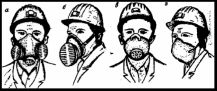
\includegraphics[]{1.jpg}
    \caption{Противопылевые респираторы: а--Астра-2; б--Ф62Ш;\\ в--УК-2М; г--ШБ-1}
    \label{fig}
\end{figure}


Респиратор ``Астра-2'' состоит из резиновой полумаски, снабженной клапаном выдоха, и двух полиэтиленовых коробок с клапанами вдоха. В коробки заложен гофрированный фильтр из материала фГТП-15. Его можно применять при температуре до -- 25° С.

Респиратор Ф62Ш состоит из резиновой полумаски с закрепленной на ней пластмассовой коробкой, в которой помещается сменный противопылевой фильтр. Коробка соединена с полумаской клапаном вдоха, в нижней части которой находится клапан выдоха.

Респиратор РП-КМ состоит из резиновой полумаски, снабженной клапанами вдоха и выдоха. По внешнему периметру маска имеет эластичную манжету, под которую вставляются и пристегиваются две фильтрующие оболочки внутренняя из материала Ф1111-15 и наружная из поролона. Благодаря клапану выдоха фильтрующие оболочки не увлажняются, меньше забиваются пылью и не затрудняют дыхание. Внутреннюю оболочку респиратора можно заменить в течение 1 мин, внешнюю промывают в воде и высушивают.

Для работающих в выработке при повышенной запыленности воздуха с большой физической нагрузкой рекомендованы респираторы Астра-2М, Ф62Ш, РП-КМ, а при выполнении легкой и средней тяжести работ — респираторы ТТТБ-1, "Леписток-5", УК-2М. В настоящее время освоены новые респираторы ПРШ 741 и РПМ-73 повышенной пылеёмкости. Эффективность пылеулавлавливания составляет 99,9\%.


\section{Ответы на контрольные вопросы}
\begin{enumerate}
    \item Какие средства защиты органов дыхания вы знаете?
    \item [Ответ:] Противогазы, респираторы, простейшие средства защиты (противопыльные тканевые маски ПТМ-1, ватно-марлевые повязки).
    \item []
    \item Как различаются респираторы по конструктивному испытанию?
    \item [Ответ:] Респираторы многоразового использования со сменными фильтрами и респираторы кратковременного (одно-, двукратного) пользования, в которых фильтрующим элементом является сама маска.
    \item []
    \item Предохраняют ли респираторы от газов?
    \item [Ответ:] Нет.
    \item []
    \item По разрешению, каких органов надзора респираторы используются как основное средство защиты?
    \item [Ответ:] Госгортехнадзор, госсанинспекция.
    \item []
    \item Какова эффективность пылеулавливания у самых современных респираторов?
    \item [Ответ:] Эффективность пылеулавлавливания составляет 99,9\%.
\end{enumerate}


\subsection*{Вывод}
В ходе выполнения данной практической работы я самостоятельно ознакомился со средствами индивидуальной и групповой защиты и ответил на контрольные вопросы.
\end{document}